\documentclass[border=10pt]{standalone}
\usepackage{pgfplots}
\usepackage{pgfplotstable}
\pgfplotsset{width=7cm,compat=1.8}
\begin{document}
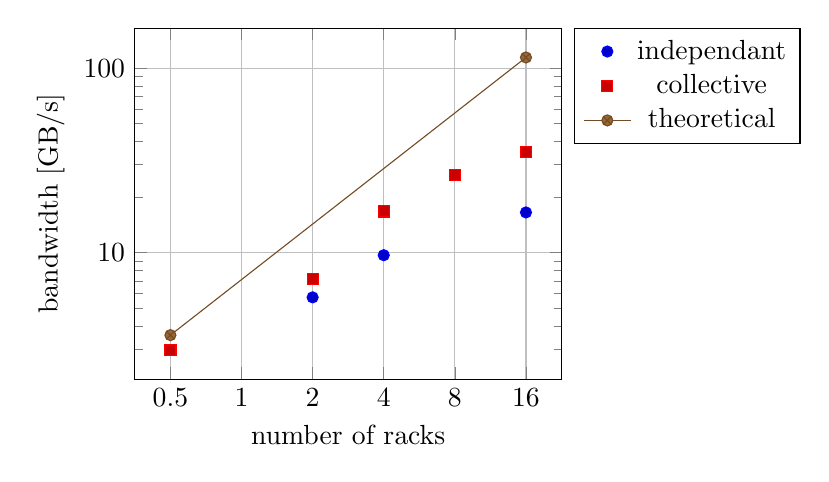
\begin{tikzpicture}
\begin{loglogaxis}[
    %title=Measured bandwidth,
    xlabel={number of racks},
    ylabel={bandwidth [GB/s]},
    ytick={1,10,100},
    yticklabels={1,10,100},
    xtick={0.5,1,2,4,8,16},
    xticklabels={0.5,1,2,4,8,16},
    grid=major,
    legend entries={independant, collective, theoretical},
    legend pos = outer north east
]
\addplot+[only marks] plot coordinates {
	(2,5.721420558) 
  	(4,9.6816671958)
  	(16,16.5156862228)};
\addplot+[only marks] plot coordinates {
	(0.5,2.9714412287)
	(2,7.2191194685) 
  	(4,16.7147588699)
  	(8,26.2716162222)
  	(16,35.1318015922)};
\addplot plot coordinates {
	(0.5,3.57) 
	(16,114.29)};
\end{loglogaxis}
\end{tikzpicture}
\end{document}